% This is lnbip.tex the demonstration file of the LaTeX macro package for
% Lecture Notes in Business Information Processing from Springer-Verlag.
% It serves as a template for authors as well.
% version 1.0 for LaTeX2e
%
\documentclass[lnbip]{svmultln}
%
\usepackage{makeidx}  % allows for indexgeneration
\usepackage{amsmath,amssymb,amsfonts}
\usepackage{graphicx}
\usepackage{textcomp}
\usepackage{xcolor}
\usepackage{booktabs}
\usepackage{algorithm}
\usepackage{algpseudocode}
\usepackage{multirow}
\usepackage{tabularx}
% \usepackage{geometry}

\usepackage{anysize}
\marginsize{4cm}{4cm}{3cm}{4cm}

\usepackage[style=ieee, backend=biber]{biblatex}
\addbibresource{references.bib}

% \makeindex          % be prepared for an author index
%

\begin{document}
%
\mainmatter              % start of the contribution
%
\title{Q-Learning-Based Load Balancing for JSON-RPC Requests in Blockchain Networks}
%
\titlerunning{Q-Learning-Based Load Balancing for JSON-RPC servers}  % abbreviated title (for running head)
%                                     also used for the TOC unless
%                                     \toctitle is used
%
\author{Ba Ngoc Nguyen\textsuperscript{\textsection} \and Tuan-Dat Trinh\textsuperscript{\textsection*[\orcidID{0000-0002-3014-3737}]}}

%
\authorrunning{B. N. Nguyen and T.-D. Trinh}   % abbreviated author list (for running head)
%
%%%% list of authors for the TOC (use if author list has to be modified)
% \tocauthor{Ivar Ekeland, Roger Temam, Jeffrey Dean, David Grove,
% Craig Chambers, Kim B. Bruce, Elisa Bertino}
%
\institute{School of Information and Communications Technology\\
Hanoi University of Science and Technology\\
\email{ngoc.mywork1819@gmail.com}\\
\email{dattt@soict.hust.edu.vn}
\footnotetext{
\textsuperscript{\textsection}The two authors contributed equally to this work.\\
\textsuperscript{*}Corresponding author.
}}

\maketitle              % typeset the title of the contribution
% \index{Ekeland, Ivar} % entries for the author index
% \index{Temam, Roger}  % of the whole volume
% \index{Dean, Jeffrey}

\begin{abstract}        % give a summary of your paper
Blockchain JSON-RPC servers play a critical role in enabling client interactions with decentralized applications. However, they face substantial load balancing challenges due to unpredictable workloads, such as transaction spikes during high-traffic events. These fluctuations result in uneven load distribution, increased latency, and reduced throughput. Traditional approaches like round-robin and least-connections fail to adapt effectively in heterogeneous blockchain environments.
This paper introduces a Q-learning-based reinforcement learning (RL) framework to dynamically balance loads across JSON-RPC servers in Ethereum Virtual Machine (EVM) networks. By formulating the problem as a Markov Decision Process (MDP), the algorithm learns optimal routing policies based on real-time server states and request types, improving both latency and load distribution.
Experiments on a locally deployed network demonstrate that our method outperforms traditional baselines. It achieves 19.61 ms average latency with zero failures under average load, boosts throughput fivefold to 1,293.72 requests per second under high load, and maintains 0.03\% failure rate with 1,600 ms P99 latency under variable conditions. These results highlight the approach’s effectiveness in enhancing scalability, reliability, and responsiveness for blockchain-based applications.
%                         please supply keywords within your abstract
\keywords {Load Balancing, Q-learning, Reinforcement Learning, JSON-RPC Servers, Blockchain.}
\end{abstract}
%
\section{Introduction}\label{s:1}
%
Blockchain technology, exemplified by Ethereum and its Ethereum Virtual Machine (EVM), has transformed decentralized applications (dApps) by enabling secure, programmable transactions without intermediaries~\cite{cai2018, pilkington2016}. At the core of this ecosystem are JSON-RPC servers, which act as gateways for client communication with blockchain nodes. These servers expose a standardized set of methods such as \texttt{eth\_getBalance} and \texttt{eth\_sendTransaction} via a lightweight, stateless protocol over HTTP or WebSocket. They handle key operations including transaction submissions, smart contract executions, and blockchain state queries, making them critical to the functionality and responsiveness of dApps. As blockchain adoption grows, ensuring the efficiency and reliability of JSON-RPC servers has become increasingly important.

Despite their central role, JSON-RPC servers face major challenges in handling dynamic and unpredictable blockchain workloads. Sudden spikes in transaction volume during high-demand events often lead to imbalanced load distribution, increased latency, and reduced throughput. Traditional load balancing methods such as round-robin and least-connections struggle to adapt to real-time variations in server load and network conditions. As a result, they hinder the scalability and responsiveness of blockchain applications, creating a performance bottleneck that limits broader adoption.

Reinforcement learning (RL) offers a promising solution to these challenges. By enabling agents to learn optimal decision-making policies through interaction with the environment, RL is well-suited for dynamic and unpredictable systems such as blockchain networks~\cite{sutton1998}. Among RL methods, Q-learning is a model-free algorithm that can adaptively route requests by learning from experience rather than relying on static heuristics. By formulating the load balancing problem as a Markov Decision Process (MDP), where states represent server loads and actions correspond to routing choices, Q-learning enables dynamic optimization of performance, effectively balancing loads and minimizing latency.

This paper presents a Q-learning-based approach for load balancing JSON-RPC requests in blockchain networks. The goal is twofold. First, we design an adaptive algorithm that dynamically routes client requests to optimize response time and throughput. Second, we evaluate its effectiveness through simulations and experiments on EVM networks.

The main contributions of this work are as follows. First, we formalize the load balancing problem for JSON-RPC servers as a Markov Decision Process, providing a structured foundation for applying reinforcement learning. Second, we design a Q-learning algorithm tailored to blockchain workloads, with a reward function that jointly optimizes latency and load distribution. Third, we demonstrate through extensive experiments that our method outperforms traditional techniques such as round-robin and least-connections in both response time and throughput. It also maintains stable performance under dynamic and fluctuating workloads.

The rest of the paper is organized as follows. Section~\ref{s:2} reviews related work on load balancing and reinforcement learning in blockchain systems. Section~\ref{s:3} introduces the system architecture and formalizes the load balancing problem. Section~\ref{s:4} presents the proposed Q-learning algorithm. Section~\ref{s:5} explains the experimental setup and reports the results. Section~\ref{s:6} analyzes the implications and limitations of the approach. Finally, Section~\ref{s:7} concludes the paper and outlines future research directions.

\section{Related Work}\label{s:2}
Load balancing is a fundamental aspect of distributed systems. It ensures efficient resource allocation and helps maintain consistent performance under dynamic workloads \cite{ivanisenko2015}.  For JSON-RPC servers that handle client interactions, effective load balancing is essential for managing dynamic request patterns and ensuring low-latency performance. This section reviews traditional load balancing techniques, explores solutions tailored to blockchain environments, and discusses the application of RL to load balancing. It also highlights the limitations of existing approaches and explains how our Q-learning-based method addresses these challenges.

Traditional load balancing strategies such as round-robin, weighted round-robin, and least-connections are widely adopted due to their simplicity and ease of implementation \cite{ibrahim2021web, jader2019state}. The round-robin method distributes incoming requests sequentially across available servers, while the weighted variant enhances this approach by assigning traffic based on server capacity, directing more requests to higher-capacity nodes \cite{gilly2011up}. However, both methods are static and fail to adapt to real-time changes in system conditions. The least-connections strategy offers a more dynamic alternative by routing requests to the server with the fewest active connections, aiming to distribute load more evenly \cite{gilly2011up}. Despite their effectiveness in stable environments, these techniques are inadequate for blockchain networks, where workloads are highly variable and can experience abrupt transaction surges during periods of peak demand.

To meet the specific load balancing needs of blockchain systems, several specialized tools have been developed. One example is dshackle \cite{emeraldpay2025}, a fault-tolerant load balancer for blockchain APIs. It distributes JSON-RPC requests to multiple blockchain nodes, commonly referred to as \textit{upstream nodes}, which handle tasks such as transaction processing and state queries. dshackle applies a round-robin strategy enhanced with factors like node location, synchronization status, and blockchain height. However, its routing remains static and does not adapt to real-time performance changes, limiting its effectiveness in dynamic environments.

Another example is dRPC \cite{ajala2024}, a decentralized Web3 infrastructure that extends dshackle with a proxy layer called Dproxy. Dproxy applies a machine learning algorithm to rank \textit{upstream nodes} based on real-time metrics such as performance, availability, and compute capacity, updating these rankings every second. Its approach relies on heuristic monitoring and reactive adjustments. While dRPC offers greater adaptability than static methods, it lacks the proactive, experience-driven decision-making capabilities that reinforcement learning can provide in volatile and rapidly changing environments.

Recent research has increasingly focused on addressing the unique load balancing challenges inherent to blockchain systems. \citeauthor{li2021} \cite{li2021} conducted a measurement study on nine real-world RPC services and identified vulnerabilities to Denial of Ethereum RPC Service (DoERS) attacks. Their findings revealed that static load balancing methods caused latency to increase by factors ranging from 2.1 to 50 under attack conditions. To address this, they proposed an “unpredictable load balancing” strategy to enhance security and emphasized the importance of adaptive and dynamic mechanisms. RL is well-suited to this context due to its ability to adjust behavior in response to real-time changes.

Following this line of research, \citeauthor{alotaibi2022} \cite{alotaibi2022} explored the use of RL for load balancing in Hyperledger Fabric, a private blockchain platform. Their method applies the Contextual Multi-Armed Bandits algorithm to monitor resource usage--including CPU, memory, and storage--and dynamically scale containers within a Docker Swarm cluster. Experimental results demonstrated the effectiveness of RL in optimizing resource allocation in controlled, private environments. However, due to the closed and centralized nature of private blockchains, this solution does not readily generalize to public blockchains, which are subject to more decentralized and unpredictable workloads.

RL has emerged as a promising approach for load balancing across other domains, including cloud computing and data centers.  \citeauthor{chawla2024} \cite{chawla2024} proposed an RL-based adaptive scheme for dynamic cloud environments, demonstrating superior performance over traditional methods. \citeauthor{park2022} \cite{park2022} applied RL to load balancing in distributed heterogeneous storage systems, while \citeauthor{ding2020} \cite{ding2020} introduced QEEC, a Q-learning framework for energy-efficient cloud computing that combines queueing models with dynamic virtual machine scheduling to reduce response time and improve CPU utilization. Although these studies highlight the flexibility and effectiveness of RL, they are not designed for blockchain systems, where decentralization and transaction-driven workloads create fundamentally different performance requirements.

Despite growing interest in RL, its application to load balancing in public blockchain systems remains limited. This gap is critical, as public blockchains demand adaptive solutions to cope with decentralized coordination and highly variable transaction loads. To address this, our work applies Q-learning, a model-free RL algorithm, to optimize load balancing for JSON-RPC servers in public blockchain networks.

\section{System Model and Problem Formulation}\label{s:3}
This section describes the architecture of a load-balanced blockchain node system that handles JSON-RPC requests and formalizes the associated load balancing problem. By modeling both the system and the decision-making process, we provide a foundation for optimizing request distribution across multiple blockchain nodes.


\subsection{System Description}\label{s:3.1}

The system architecture comprises three main layers, as illustrated in Fig.~\ref{fig:load-balancing-architecture}. At the first layer, clients including dApps, web interfaces, and end users send JSON-RPC requests to perform tasks such as querying blockchain data, submitting transactions, or invoking smart contracts. The second layer is a central load balancer that routes these requests based on real-time performance metrics. It prevents bottlenecks, distributes workload efficiently, and optimizes resource usage across the system. The third layer includes multiple blockchain nodes, each providing an RPC interface to handle incoming requests. This multi-node setup ensures scalability and stable performance, even under high or fluctuating traffic.

\begin{figure}[htbp]
    \centering
    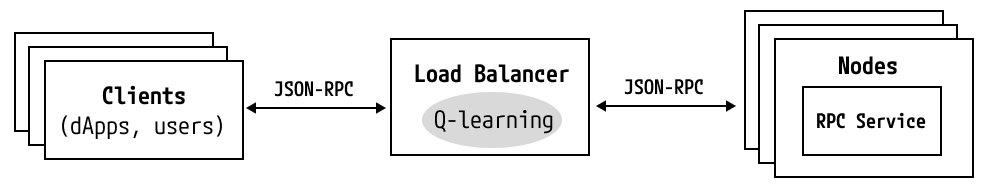
\includegraphics[width=0.75\linewidth]{load_balancing_architecture.png}
    \caption{Overview of the Load Balancing System}
    \label{fig:load-balancing-architecture}
\end{figure}
%
Each node runs independently and manages its own computational resources, including CPU, memory, and storage. The load balancer continuously monitors the state of all nodes and makes routing decisions in real time. This architecture improves scalability, fault tolerance, and responsiveness, which are critical for blockchain applications that require high reliability and low latency.


\subsection{Problem Statement and Objectives}\label{s:3.2}

Designing an intelligent load balancing strategy for blockchain JSON-RPC servers presents significant challenges. The strategy focuses on three main objectives to improve system efficiency. First, it aims to minimize latency by reducing the average response time for client requests, thereby improving user experience and minimizing delays in transaction processing or data retrieval. Second, it seeks to maximize throughput by increasing the number of requests processed per unit time. This objective requires efficient utilization of all $N$ nodes, especially during peak traffic. Third, it ensures balanced load distribution by allocating workloads evenly across nodes. This prevents performance degradation caused by overloading individual nodes and helps maintain system stability.


The load balancer must route each incoming request to the most appropriate node by considering both the request's computational complexity and the current state of each node. This decision-making process becomes more challenging due to the stochastic nature of request arrivals and processing times. To maintain optimal system performance under varying conditions, the strategy must rely on an adaptive and data-driven approach.


\subsection{Markov Decision Process formulation}\label{s:3.3}

This section formulates the load balancing problem as a Markov Decision Process (MDP), which provides a principled framework for sequential decision-making under uncertainty~\cite{puterman1990}.

\subsubsection{State}\label{s:3.3.1}
We define the system state using a finite set $\mathcal{S}$. Each state $s \in \mathcal{S}$ describes the system condition at the time a new request arrives, as shown in~\eqref{eq:state-definition}. The variable $m$ indicates the type of the request and reflects its computational complexity. The term $l_i$ denotes the current workload of node $i$, representing the load distribution across all $N$ nodes.

\begin{equation}
s = (m, l_1, l_2, \ldots, l_N)
\label{eq:state-definition}
\end{equation}

By including $m$, the load balancer can account for computational complexity. For example, a \texttt{eth\_getBalance} request is lightweight, while executing a smart contract requires more resources. This distinction allows the balancer to assign simple requests to lightly loaded nodes and reserve capacity for heavier tasks.

Workload levels $l_i$ directly influence node performance. Overloaded nodes may increase latency or fail to respond, while underutilized nodes reduce system efficiency. Tracking $l_i$ helps balance the load and minimize response times.

Treating $l_i$ as a continuous value (e.g., exact workload percentage) results in an infinite state space, making Q-learning computationally infeasible. Even if we apply a fine-grained discretization, the state space still grows rapidly. Let $M$ denote the number of request types and $N$ the number of nodes. If each node has 100 discrete workload levels, then the total number of states becomes $M \times 100^N$. For example, with $M = 5$ and $N = 3$, the state space reaches $5 \times 100^3 = 5{,}000{,}000$. This exponential growth leads to the curse of dimensionality~\cite{bellman1957}, where the learning process becomes inefficient due to the large number of possible states.

To address this, we adopt a coarse discretization strategy, reducing $l_i$ to $L$ levels. Using $L = 3$ and defining ranges as Low ($0\%$–$33\%$), Medium ($33\%$–$66\%$), and High ($66\%$–$100\%$), the state space reduces to $M \times 3^N$. With $M = 5$ request types and $N = 3$ nodes, the total number of states becomes $5 \times 3^3 = 135$. This simplification improves computational efficiency while preserving key characteristics of load distribution.


\subsubsection{Actions}\label{s:3.3.2}

The action space $\mathcal{A} = \{1, 2, \ldots, N\}$ represents the set of routing options available to the load balancer, where action $a = i$ assigns the request to node $i$. Since the number of actions equals the number of nodes, the action space is discrete, compact, and easy to compute.


\subsubsection{Rewards}\label{s:3.3.3}
The reward function $R(s, a, s')$ evaluates the quality of routing a request to a specific node via action $a$, which causes the system to transition from state $s$ to state $s'$. It is designed to support two primary objectives: minimizing latency and ensuring balanced load across nodes, thereby improving overall throughput.

The latency component encourages actions that reduce response time, which is essential for improving user experience. It is typically defined as an inverse function, such as $\frac{{latency}_{scale}}{{latency}}$ or $\frac{1}{{latency}}$, where $latency$ is measured in milliseconds and ${latency}_{scale}$ (e.g., 50 ms) serves as a normalization factor. This formulation yields higher rewards for faster responses while keeping the metric dimensionless and comparable. For instance, a $latency$ of 25 ms results in a reward of 2, whereas 100 ms yields 0.5 when ${latency}_{scale} = 50$.

However, relying solely on latency can overload the fastest node. Over time, this increases its queue length and degrades performance, while other nodes remain underutilized. The resulting imbalance reduces system scalability and stability. To avoid this, the reward function must also account for load distribution.

To address the shortcomings of a latency-only reward, a load balance component is incorporated to discourage uneven workload distribution. This component is defined as $\frac{1}{1 + k (\max_i l_i' - \min_i l_i')}$, where $\max_i l_i'$ and $\min_i l_i'$ denote the maximum and minimum node workloads in the next state $s'$, and $k$ is a weighting factor that controls the penalty for imbalance. When workloads are similar across nodes, the term approaches 1, resulting in a higher reward. For example, if all nodes are equally loaded, $\frac{1}{1 + 0.1 \times 0} = 1$. Conversely, significant disparities reduce the reward, such as $\frac{1}{1 + 0.1 \times 50} = \frac{1}{6} \approx 0.167$, thereby discouraging routing decisions that increase imbalance.

To account for request failures caused by node overload or hardware issues, a penalty term is introduced. This negative reward discourages actions that exceed node capacity, thereby promoting system reliability, especially under high demand.
The complete reward function is defined in~\eqref{eq:reward}. When a request is successfully processed, the reward is the product of a latency-based term and a load balance term. If the request fails, a fixed penalty is applied.

\begin{equation}
    \scriptsize
    \label{eq:reward}
    R(s, a, s') =
    \begin{cases}
        \dfrac{{latency}_{{scale}}}{{latency(1 + k(\max_i l_i' - \min_i l_i'))}} & \text{if request succeeds} \\
        {penalty} & \text{if request fails}
    \end{cases}
\end{equation}

The composite reward function balances the trade-off between latency and load distribution. By penalizing imbalance, it prevents the agent from overloading a single node, while still incentivizing fast responses. The parameters ${latency}_{{scale}}$ and $k$ can be tuned to emphasize either latency reduction or load balancing, depending on system requirements.


\subsubsection{Transition Probabilities}\label{s:3.3.4}

The transition probability $P(s' | s, a)$ represents the likelihood of the system moving to state $s'$ after action $a$ is taken in state $s$. These transitions are inherently stochastic, influenced by request arrival patterns (e.g., modeled as a Poisson process) and processing times, which depend on the request type $m$ and the load $l_i$ of each node. Although exact probabilities are difficult to model, the MDP framework leverages observed state transitions and rewards, allowing learning to proceed without an explicit transition model.


\section{Proposed Method}\label{s:4}

We adopt Q-learning, a model-free reinforcement learning algorithm, to solve the MDP and derive an optimal load balancing policy. Q-learning is well suited for dynamic environments, as it learns directly from real-time interactions without requiring a model of the system.

The Q-table $Q: \mathcal{S} \times \mathcal{A} \to \mathbb{R}$ stores the expected cumulative reward for each state-action pair and is initialized to zero. Given $M$ request types, $N$ nodes, and $L$ discrete load levels, the table contains $M \times L^N \times N$ entries. The size of the state space can be controlled by selecting an appropriate value for $L$.

For each incoming request, the current state $s$ is observed based on the request type $m$ and the discrete load levels $(l_1, ..., l_N)$ of all nodes, i.e., $s = (m, l_1, ..., l_N)$. To balance exploration and exploitation, the algorithm employs an $\varepsilon$-greedy policy \cite{sutton1998}. With probability $\varepsilon$, it selects a random action to explore alternative routing decisions; with probability $1 - \varepsilon$, it selects the action $a = \arg\max_{a'} Q(s, a')$ that yields the highest estimated reward.

At the beginning of training, a high exploration rate (e.g., $\varepsilon = 1.0$) promotes broad exploration of the action space and helps prevent early convergence to suboptimal policies. As learning progresses, $\varepsilon$ gradually decays toward a predefined minimum $\varepsilon_\text{min}$ after every $\varepsilon_\text{decaySteps}$ steps, following the update rule in~\eqref{eq:epsilon_decay}.
This adaptive decay strategy gradually shifts the load balancer’s focus from exploration to exploitation, allowing it to leverage the increasingly accurate Q-values. At the same time, it retains a degree of exploration to accommodate potential changes in server performance, enabling continuous adaptation and improved decision-making over time.


\begin{equation}
    \varepsilon = \max(\varepsilon_\text{min}, \varepsilon \times \varepsilon_{\text{decayRate}})
    \label{eq:epsilon_decay}
\end{equation}

After routing a request to node \( a \), the balancer observes the immediate reward \( r = R(s, a, s') \) and transitions to the next system state \( s' \). The Q-value corresponding to the state-action pair \( (s, a) \) is then updated using the Bellman equation \cite{bellman1957}, as shown in~\eqref{eq:q_update}. Here, \( \alpha \) denotes the learning rate, which determines the extent to which new information overrides prior knowledge, while \( \gamma \) represents the discount factor, controlling the relative importance of future versus immediate rewards.

\begin{equation}
    Q(s, a) \gets Q(s, a) + \alpha \left[r + \gamma \max_{a'} Q(s', a') - Q(s, a)\right]
    \label{eq:q_update}
\end{equation}

This iterative update allows the balancer to refine its Q-values over time based on real-time feedback, progressively improving its routing policy. The complete Q-learning procedure is summarized in Algorithm~\ref{algo:qlearning}.

\begin{algorithm}
\footnotesize
\caption{Q-Learning for Load Balancing}
\label{algo:qlearning}
\begin{algorithmic}[1]
\Statex \textbf{Input:}
\Statex Learning rate $\alpha$, discount factor $\gamma$
\Statex Exploration parameters: $\varepsilon$, $\varepsilon_{\min}$, $\varepsilon_{\text{decayRate}}$, $\varepsilon_{\text{decaySteps}}$
\Statex Load imbalance weight $k$, number of load levels $L$
% \vspace{1mm}

\State Initialize $Q(s, a) \gets 0$ for all $s \in \mathcal{S}, a \in \mathcal{A}$
\State Set $steps \gets 0$
% \vspace{1mm}

\For{each incoming request}
    \State $steps \gets steps + 1$
    \State Observe current state $s \gets (m, l_1, \dots, l_N)$
    \State Select action $a$ using $\varepsilon$-greedy policy based on $Q(s, a)$
    \State Route request to node $a$
    \State Observe reward $r = R(s, a, s')$ and next state $s'$
    \State Update $Q(s, a)$ using Equation~\ref{eq:q_update}
    \If{$\text{mod}(steps, \varepsilon_{\text{decaySteps}}) = 0$}
        \State $\varepsilon \gets \max\left(\varepsilon_{\min}, \varepsilon \times \varepsilon_{\text{decayRate}}\right)$
    \EndIf
\EndFor
\end{algorithmic}
\end{algorithm}

\section{Experimental Evaluation}\label{s:5}

\subsection{Experimental Setup}\label{s:5.1}

To ensure a controlled and reproducible environment, all experiments were performed on a locally deployed EVM blockchain network using Docker containers \cite{merkel2014docker}. The host system was a high-performance workstation running Windows OS, equipped with an AMD Ryzen 9 5900X 12-core processor (3.7 GHz), 32~GB of RAM, and a 1~TB SSD.

Four Ethereum client implementations were selected based on usage statistics reported by the Ethereum Node Tracker\footnote{\url{https://etherscan.io/nodetracker}}, including Geth\footnote{\url{https://github.com/ethereum/go-ethereum}}, Nethermind\footnote{\url{https://github.com/NethermindEth/nethermind}}, Reth\footnote{\url{https://github.com/paradigmxyz/reth}}, and Erigon\footnote{\url{https://github.com/erigontech/erigon}}. Each client was allocated dedicated hardware resources, as specified in Table~\ref{t:es_2}, to eliminate performance interference and simulate diverse node configurations.

Prior to testing, we benchmarked each node to determine its processing capacity, defined as the highest request rate that a node can sustain while keeping the error rate below 1\%. This preliminary step ensured that subsequent load balancing evaluations were conducted under realistic and capacity-aware conditions.

The experiment analyzed JSON-RPC request patterns based on the JSON-RPC 2.0 Specification\footnote{\url{https://www.jsonrpc.org/specification}}, focusing on 21 core methods categorized into three functional groups\footnote{\url{https://ethereum.org/en/developers/docs/apis/json-rpc/}}: \textit{gossip}, \textit{state}, and \textit{history}. A synthetic workload was constructed to emulate realistic Ethereum mainnet behavior, with requests proportionally distributed across these categories to reflect typical usage patterns.

To evaluate system performance under varying workload intensities, the synthetic traffic was applied across three distinct test scenarios, as outlined in Table~\ref{t:es_1}. The experiments were executed using Grafana k6\footnote{\url{https://grafana.com/docs/k6/next/}}, an open-source load testing tool. Each virtual user was configured to issue one request per second in a sequential manner. The three scenarios reflect typical operational conditions: steady average load, sustained high traffic, and dynamically fluctuating request rates.

\begin{table}[htbp]
\caption{Resource configuration of blockchain nodes}
\begin{center}
    \begin{tabular}{|c|c|c|c|}
        \hline
        \textbf{Node ID} & \textbf{Client} & \textbf{Memory} & \textbf{Capacity (req/s)} \\
        \hline
        Node 1 & Geth       & 2048 MB & 320 \\
        Node 2 & Nethermind & 3072 MB & 340 \\
        Node 3 & Reth       & 2048 MB & 320 \\
        Node 4 & Erigon     & 4096 MB & 350 \\
        \hline
    \end{tabular}
    \label{t:es_2}
\end{center}
\end{table}

\begin{table}[htbp]
\caption{Load testing scenarios}
\begin{center}
    \begin{tabular}{|l|c|c|}
        \hline
        \textbf{Scenario} & \textbf{Concurrent Users} & \textbf{Duration (min)} \\
        \hline
        Average load   & 300           & 40 \\
        High load      & 1600          & 40 \\
        Variable load  & 300 -- 4000   & 42 \\
        \hline
    \end{tabular}
    \label{t:es_1}
\end{center}
\end{table}

\begin{table}[htbp]
\caption{Q-learning hyperparameter settings}
\begin{center}
    \begin{tabular}{|l|c|l|c|}
        \hline
        \textbf{Parameter} & \textbf{Value} & \textbf{Parameter} & \textbf{Value} \\
        \hline
        Learning rate $\alpha$         & 0.1   & Exploration rate $\epsilon$       & 1.0   \\
        Discount factor $\gamma$       & 0.95  & Min exploration $\epsilon_{min}$ & 0.01  \\
        Discrete load levels $L$       & 8     & Decay rate $\epsilon_{decayRate}$ & 0.995 \\
        Imbalance weight $k$           & 3     & Decay steps $\epsilon_{decaySteps}$ & 300 \\
        Failure penalty                & -2    &                                   &       \\
        \hline
    \end{tabular}
    \label{t:es_3}
\end{center}
\end{table}

The proposed Q-learning-based load balancing method was comprehensively evaluated against two baseline techniques: round-robin and least-connections. The algorithm's hyperparameters were carefully tuned to enhance its learning efficiency and responsiveness under dynamic workloads, as detailed in Table~\ref{t:es_3}. 

Performance was assessed using four primary metrics: total number of processed requests, throughput (measured in requests per second), failure rate (percentage of failed requests), and request latency including average, 95th percentile (P95), and 99th percentile (P99) values.

\subsection{Experimental Results}\label{s:5.2}
Tables~\ref{t:ex_1}, \ref{t:ex_2}, and \ref{t:ex_3} summarize the results under three scenarios: average, high, and variable loads. Across all settings, the Q-learning approach consistently outperforms traditional methods in throughput, latency, and failure rate. Q-learning achieves the highest throughput, ranging from 617{,}709 to 3{,}105{,}558 processed requests, with sustained speeds between 257.28 and 1{,}293.72 requests per second. It also maintains excellent reliability, with a failure rate between 0\% and 0.03\%, and demonstrates fast response times, with average latency from 19.61~ms to 125.71~ms and 99th percentile latency (P99) between 130.52~ms and 1{,}600~ms.

\begin{table}[htbp]
\centering
% \begin{minipage}{\columnwidth}
\caption{Performance comparison under average load}
% \resizebox{\columnwidth}{!}{
\setlength{\tabcolsep}{5pt}
\begin{tabular}{lccccccc}
\toprule
\textbf{Algorithm} & \textbf{Total} & \textbf{Throughput} & \textbf{Failures} & \multicolumn{3}{c}{\textbf{Request Duration (ms)}} \\
 & \textbf{Requests} & \textbf{(req/s)} & \textbf{(\%)} & \textbf{Avg} & \textbf{P95} & \textbf{P99} \\
\midrule
\textbf{Q-learning} & \textbf{617{,}709} & \textbf{257.28} & \textbf{0.00} & \textbf{19.61} & \textbf{28.71} & \textbf{130.52} \\
Round-robin & 598{,}926 & 249.47 & 0.00 & 51.17 & 140.47 & 798.95 \\
Least-connections & 605{,}628 & 252.26 & 0.00 & 39.60 & 123.55 & 510.58 \\
\bottomrule
\end{tabular}
% }
\label{t:ex_1}
\end{table}

\begin{table}[htbp]
\centering
\caption{Performance comparison under high load}
\setlength{\tabcolsep}{5pt}
% \resizebox{\columnwidth}{!}{
\begin{tabular}{lccccccc}
\toprule
\textbf{Algorithm} & \textbf{Total} & \textbf{Throughput} & \textbf{Failures} & \multicolumn{3}{c}{\textbf{Request Duration (ms)}} \\
 & \textbf{Requests} & \textbf{(req/s)} & \textbf{(\%)} & \textbf{Avg} & \textbf{P95} & \textbf{P99} \\
\midrule
\textbf{Q-learning} & \textbf{3{,}105{,}558} & \textbf{1{,}293.72} & \textbf{0.00} & \textbf{81.34} & \textbf{341.19} & \textbf{626.27} \\
Round-robin & 2{,}617{,}700 & 1{,}090.25 & 0.15 & 283.14 & 1{,}190 & 4{,}790 \\
Least-connections & 2{,}835{,}831 & 1{,}181.25 & 0.10 & 184.56 & 703.79 & 3{,}150 \\
\bottomrule
\end{tabular}
% }
\label{t:ex_2}
\end{table}


\begin{table}[htbp]
\centering
\caption{Performance comparison under variable load}
% \renewcommand{\arraystretch}{1.2}
% \resizebox{\columnwidth}{!}{
\setlength{\tabcolsep}{5pt}
\begin{tabular}{lccccccc}
\toprule
\textbf{Algorithm} & \textbf{Total} & \textbf{Throughput} & \textbf{Failures} & \multicolumn{3}{c}{\textbf{Request Duration (ms)}} \\
 & \textbf{Requests} & \textbf{(req/s)} & \textbf{(\%)} & \textbf{Avg} & \textbf{P95} & \textbf{P99} \\
\midrule
\textbf{Q-learning} & \textbf{2{,}535{,}101} & \textbf{1{,}005.81} & 0.03 & \textbf{125.71} & \textbf{680.11} & \textbf{1{,}600} \\
Round-robin & 2{,}224{,}641 & 882.64 & \textbf{0.03} & 283.77 & 1{,}580 & 3{,}060 \\
Least-connections & 2{,}270{,}663 & 900.77 & 0.03 & 257.19 & 1{,}370 & 2{,}240 \\
\bottomrule
\end{tabular}
% }
\label{t:ex_3}
\end{table}

In terms of scalability, Q-learning shows strong performance as the system transitions from average to high load, achieving a fivefold increase in throughput without any failure. It also remains stable under variable conditions. In contrast, round-robin exhibits a 0.15\% failure rate under high load and poor response times, with P99 latency reaching up to 4{,}790~ms. The least-connections strategy performs adequately under average load but degrades under high load, with P99 latency rising to 3{,}150~ms.
Overall, Q-learning delivers consistently low latency and robust performance, while traditional baselines fail to adapt under increasing or fluctuating demand.

\section{Discussion}\label{s:6}
The experimental results demonstrate that Q-learning consistently outperforms traditional load balancing methods, including round-robin and least-connections, across all tested scenarios: average, high, and variable loads. Its advantage stems from the ability to learn optimal routing strategies through reinforcement learning. By leveraging real-time feedback, Q-learning continuously refines its decisions to maximize long-term rewards. This leads to lower response times and failure rates, particularly under high or fluctuating workloads.

These findings offer practical value for blockchain developers and node operators. Integrating Q-learning into load balancing improves node reliability and responsiveness, which is critical for latency-sensitive applications such as DeFi and blockchain gaming. Lower latency and failure rates enhance user experience, while the algorithm's adaptability enables efficient resource usage. This reduces the need for over-provisioned hardware during traffic spikes, ultimately lowering operational costs.

Despite its strengths, Q-learning has several limitations. One key challenge is convergence time; in large or rapidly changing environments, the algorithm may require many iterations to learn an effective policy, leading to suboptimal performance during early stages. Moreover, although experiments with four Ethereum clients demonstrate promising scalability, its effectiveness in larger networks remains uncertain due to the exponential growth of the state-action space. To address this, future work may explore advanced exploration strategies or dimensionality reduction techniques to maintain efficiency at scale.

\section{Conclusion and Future Work}\label{s:7}
This study addresses the challenge of load balancing JSON-RPC requests in blockchain networks, where methods such as round-robin and least-connections often struggle to maintain performance under dynamic traffic conditions. We propose a Q-learning-based reinforcement learning approach that adaptively distributes requests across nodes based on real-time system feedback. Experimental results across average, high, and variable load scenarios show that the method improves throughput, reduces latency, and enhances network resilience. To the best of our knowledge, this is the first application of Q-learning to JSON-RPC load balancing, providing a scalable and adaptive framework for blockchain infrastructure.

% While the results are promising, several directions remain for future work. Deep Q-learning could improve scalability by approximating Q-values with neural networks, enabling faster convergence in large state spaces. Incorporating node-level metrics such as CPU usage, memory consumption, and network bandwidth into the reward function may further refine routing decisions under heterogeneous resource constraints. Additionally, hybrid approaches that combine Q-learning with supervised learning could reduce training time by bootstrapping from historical data, enhancing adaptability in highly dynamic environments.

While the proposed approach demonstrates promising results, several important directions remain for future work. A principled method for identifying optimal hyperparameters should be developed and systematically evaluated, instead of relying primarily on manual trial-and-error, in order to improve reproducibility and reduce the time required for parameter tuning. Incorporating node-level metrics such as CPU utilization, memory consumption, and network bandwidth into the reward function may further enhance routing decisions under heterogeneous resource constraints. Moreover, advanced techniques such as Deep Q-learning \cite{pmlr-v120-yang20a} can be applied to approximate the Q-function in the large state spaces arising from these extensions, thereby improving convergence speed and generalization capability in complex and highly dynamic environments.

\printbibliography

% \clearpage
\vspace{0.5cm}

\textbf{Authors' Background}

\vspace{0.25cm}

{
\setlength{\tabcolsep}{4pt}
\renewcommand{\arraystretch}{1.4}
\begin{tabularx}{\textwidth}{|l|X|X|X|}
\hline
\small
\textbf{Your Name} &
\textbf{Title} &
\textbf{Email} &
\textbf{Research Field} \\
% \textbf{Personal website} \\
\hline
Ba Ngoc Nguyen & Master student  & ngoc.mywork1819@\allowbreak gmail.com & \\
\hline
Dat-Tuan Trinh & Senior lecturer & dattt@soict.hust.\allowbreak edu.\allowbreak vn & Semantic Web, Blockchain, LLM, Logistics \\
\hline
\end{tabularx}
}

% \vspace{0.3cm}

% {\footnotesize
% *Title can be chosen from: master student, PhD candidate, assistant professor,
% lecturer, senior lecturer, associate professor, full professor
% }

\end{document}
